In order to analyze the performance of our approach proposed in this
paper, we developed a simulator to compare our work against a
clustering approach proposed for a centralized network
\cite{muruganathan2005centralized} and a distributed censoring
approach proposed in \cite{rago1996censoring}.  The sensor network on
which we conducted experiments consists of sensor nodes that are
static and homogeneous, and there is only one static CN which has
access to an unlimited amount of energy. We also assume that nodes are
deployed randomly, forming a high-density network. Performance is
measured by the quantitative metrics of amount of information gathered
and the number of transmissions taken to gather this
information. Plotting graphs using these two measures will not only
tell us about the information being gathered but will also demonstrate
the energy-efficiency of the models in consideration. This is because
energy consumption is proportional to the number of transmissions
performed \cite{torres2006energy}.

To show the results, we made use of two data sets.  First, we use a
data set collected from a simple single-hop wireless sensor network
deployment of four TelosB sensors \cite{suthaharan2010labelled}. The
data consists of humidity and temperature measurements collected
during a 6-hour period at intervals of 5 seconds. Second, the Intel
Research Lab data \cite{BodikGuestrinEtAl2004} contains data collected
from 54 sensors deployed in the Intel Research Lab measuring several
factors such as humidity, temperature, light etc.  Only the
measurements of temperature were considered from both these data sets.

\begin{figure}
\begin{center}
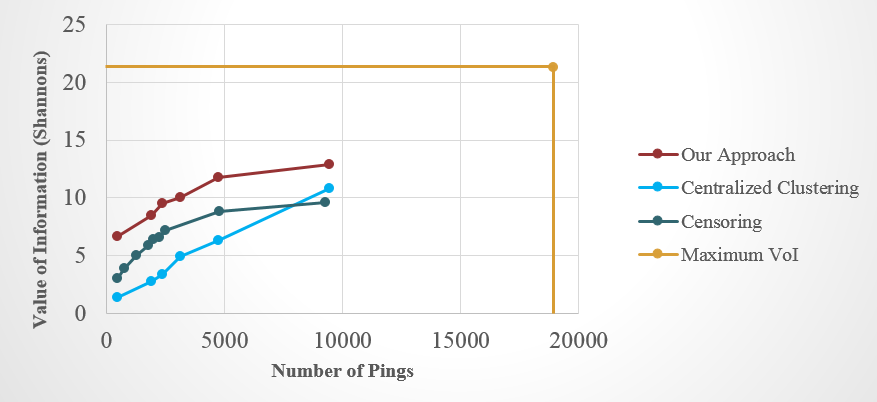
\includegraphics[height = 80mm, width = 120mm, scale = 2]{figs/Result1}
\caption{Information gathered vs Number of pings \textemdash TelosB sensor data}
\label{telosb}
\end{center}
\end{figure}
%INSERT FIGURE 4.1
\begin{figure}
\begin{center}
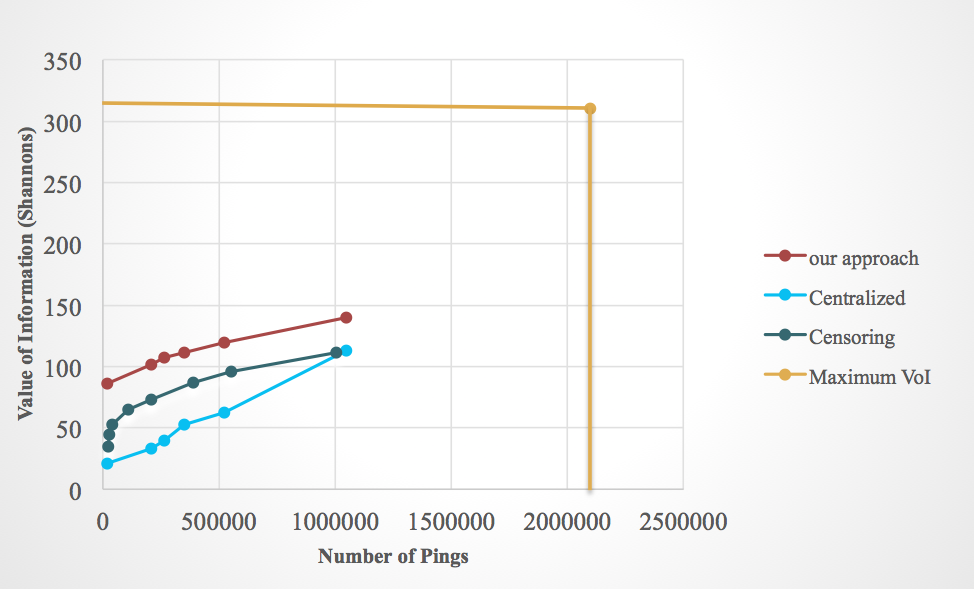
\includegraphics[height = 80mm, width = 120mm, scale = 2]{figs/Result2}
\caption{Information gathered vs Number of pings \textemdash Intel Research Lab data}
\label{intel}
\end{center}
\end{figure}
%INSERT FIGURE 4.2
In the first experiment, we considered data from the TelsoB sensors
\cite{suthaharan2010labelled}, and as stated in the algorithm above,
we calculate the entropies for each measurement of this data using
entropy equation. Next, we calculate the TM\textsubscript {VoI}
available in the data set using Algorithm \ref{tmvoi}. This will help
us understand how each model will rank against the overall information
available in the network. Next, using Algorithm
\ref{sensor-selection}, we run the simulator with this data set by
varying the number of pings. The variation in pings gives us a measure
of how each model is performing at different rates of sampling.
Obviously, the more a network is sampled, the more information can be
collected, but when we are dealing with networks that are on an energy
budget, we cannot afford sensors that perform excessive transmissions,
as it would deplete the network much faster than expected.

Figure \ref{telosb} illustrates the performance of all the models in
consideration, in terms of the amount of information gathered at
different ping rates for data gathered by the TelosB sensors in
\cite{suthaharan2010labelled}. We can clearly see that our model
outperforms both the models at each variation of the ping rate. In our
second experiment, we considered the Intel Lab data
\cite{BodikGuestrinEtAl2004}, and followed the same procedure outlined
in Section \ref{methodology}: initially determining the theoretical
maximum VoI available in a system and later choosing the informative
sensors using algorithm \ref{sensor-selection}. From Figure
\ref{intel}, we again notice our model gathering more information at
every variation in the ping rate, compared to the other two models.

Now, let us take a look at the reasons behind the performance
variation and why our model would be an ideal implementation in order
to increase the amount of information being gathered. Although both
the models chosen for comparison intend to increase the per-ping
information gathered while reducing the number of transmissions, they
were developed with the intent of discarding the information gathered
by sensors in most cases. Considering
\cite{muruganathan2005centralized}, the cluster head (CH), after
gathering information from each sensor within the cluster, performs
data aggregation and discards most of the data, sending only part of
the information gathered.  Moreover, this approach consumes extra
transmissions at every time step, as each CH again needs to transmit
information to the sink. \cite{rago1996censoring} on the other hand,
uses Likelihood Ratio (LR, defined as the dual of the ratio of the probability of
false positives and false negatives.) %%%%% IMPORTANT: DEFINE LR BEFORE USING ACRONYM %%%%% 
to transmit information to the sink. Sensors found to have LR with enough
information report information to the sink node.  Our experiments
showed that there were many instances where LR was found to be low which
resulted in excessive transmissions. Also, implementing such a decentralized 
model means that sensors will have to deal with the problems reviewed in 
Section \ref{intro}.  We also feel that if the computed LR were quantized, 
the information gathered would be higher for this approach than computed. The 
performance of our model is entirely dependent on the probability model proposed 
in Section \ref{methodology}. The algorithm, at every time step, is able to choose 
particularly informative sensors, thereby gathering more information on comparison
to other models.

The following implication can also be made from the graphs. As we
know, more information can be gathered from a network if it is sampled
more often, meaning that one would expect to see an asymptotic graph
with the previous statement taken into consideration. This can be seen
in all of the models in both of the experiments.

\begin{figure}
\begin{center}
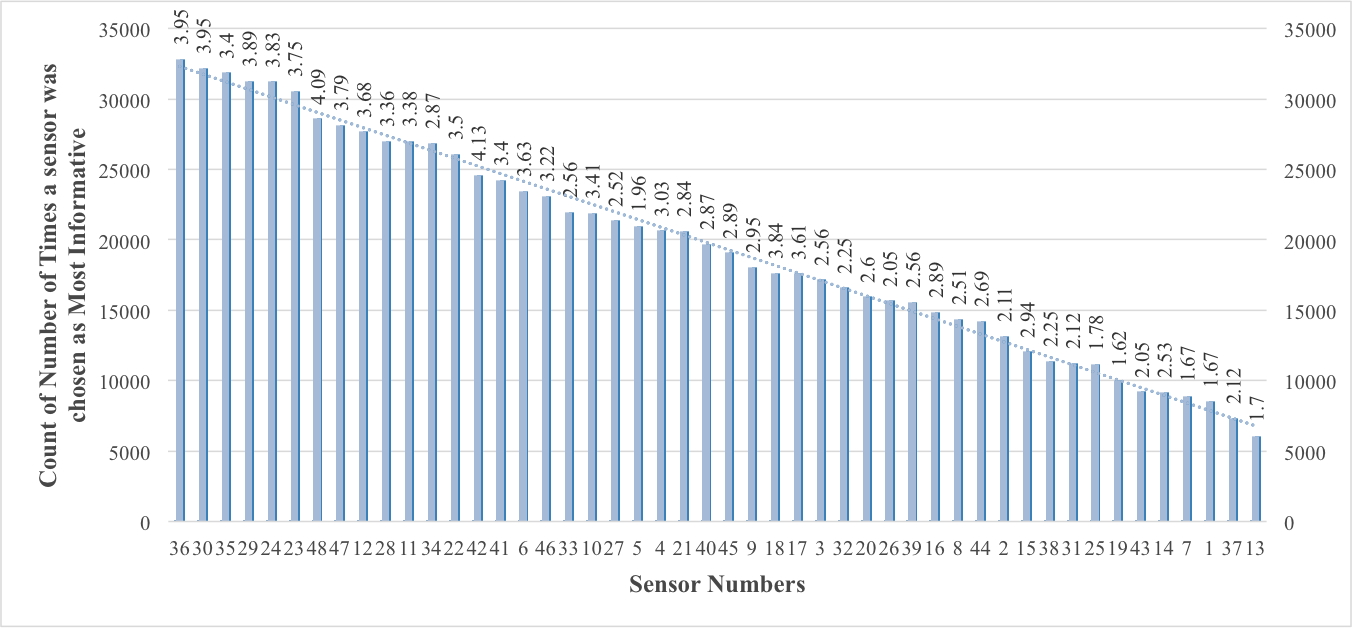
\includegraphics[height = 100mm, width = 150mm, scale = 1]{figs/Result3}
\caption{Ranking of the sensors according to the number of times chosen as Most-Informative}
\label{most-informative}
\end{center}
\end{figure}
% INSERT FIGURE 4.3
In our third experiment, we considered the Intel data set, and queried
all of the 48 sensors considered by slowing the ping rate down to 1/2
of the original.  This ping rate was chosen as a good illustration of
the network performance in terms of the amount of information
gathered. A graph was then plotted against individual sensors and the
number of times each sensor was chosen at different time steps. Figure
\ref{most-informative} shows the ranking of the sensors (from left to
right) in terms of the number of times each sensor was selected for
querying. This plot shows the consistency of the model in choosing the
sensors at each instant. Figure \ref{most-informative} is further
proof to the results above that our model correctly queries sensors at
an appropriate rate, given the amount of information predicted for
each sensor. We can also observe that the sensors gathered a
proportional amount of information with respect to the times they were
sampled. For example, sensor 36, which was chosen highest times
(approx. 32000) gathered close to 4 Shannons of information, while
sensor 26 gathered 2.05 Shannons over approximately 17000 samples.
The trend line in the graph shows the average number of queries sent
to each sensor.
%INSERT FIGURE 4.4
\begin{figure}
\begin{center}
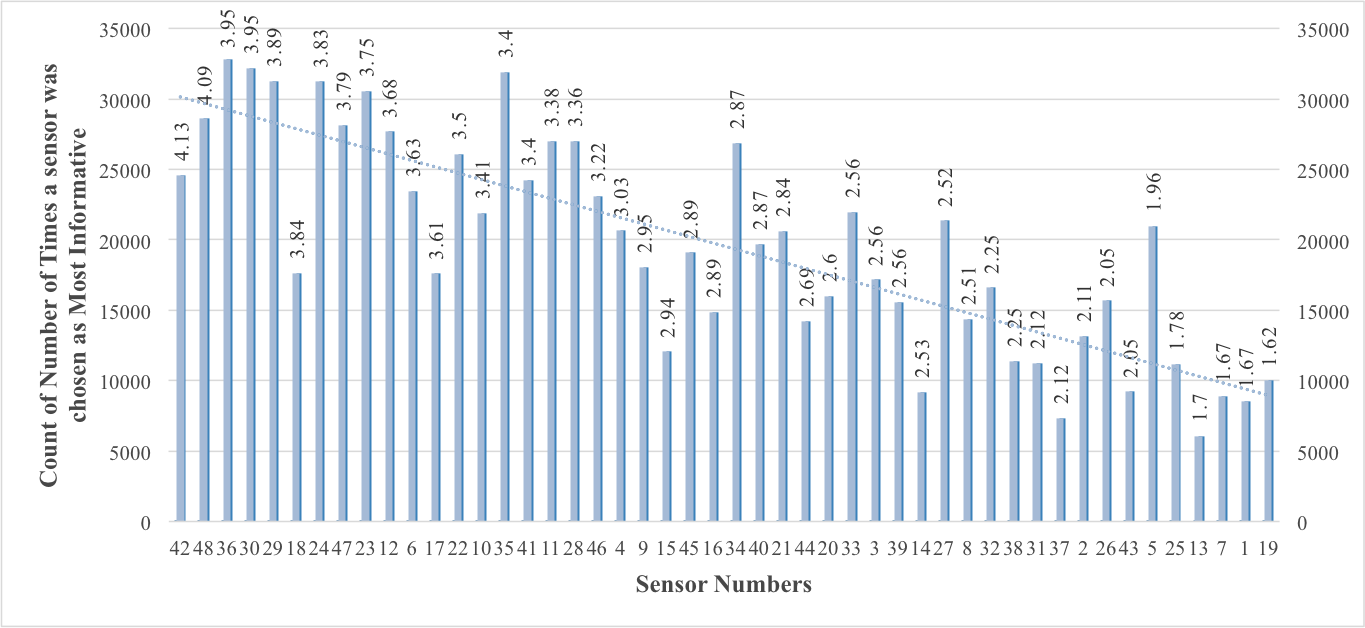
\includegraphics[height = 100mm, width = 150mm, scale = 1]{figs/Result4}
\caption{Ranking of the sensors according to amount of Information Gathered}
\label{info-gathered}
\end{center}
\end{figure}

In our final experiment, considering the same assumptions as in our
previous experiment, we plot a graph against sensor number and the
times each sensor was chosen as most informative but, this time to show
the overall VoI gathered by them. Figure \ref{info-gathered} shows the ranking
of the sensors (from left to right) in terms of the amount of information gathered
by them during a run. Our model always randomly selects a sensor based on
the current VoI gathered, not on the theoretical maximum VoI (which is not
accessible to an on-line algorithm). If that were the case, we would
have seen a result similar to figure \ref{most-informative}. However,
as the VoI distribution changes constantly with every query at every
time step, we do not see a smooth slanting curve. For the same reason,
we can also observe that certain sensors have been queried less often,
although in the end they provided a greater amount of information, and
vice-versa. However, the trend line in the graph is proof that, sensor selection
is proportional to the number of times each sensor is being queried. It also
shows the average amount of information gathered by each sensor. From
these analyses, we can clearly see how our model outperforms other state-of-the-art models,
both in terms of information collection and energy efficiency.